

One of the main research interests of our workgroup at the University of L'Aquila is the mining of open source repositories, such as \GH, to support developers. %In recent years, we have obtained encouraging results. 
As a base for further presentation, this section summarizes the main results we have obtained so far on the topic of bias in recommender systems for mining third-party libraries (TPLs). %; and \emph{(ii)} Adversarial attacks to RSSEs.%\footnote{Our work has been published in proceedings of top-tier venues including one Rank A* and two Rank A conferences.}
%\vspace{-.4cm}

% RSSEs.

%Through systematic literature reviews, we demonstrate that our work is different ...



%=============================
%\begin{itemize}
%	\item Adversarial attacks to recommender systems in Software Engineering (libraries, TPLs).
%	\item RSSE are subject to bias.
%\end{itemize}
%=============================




%=============================================
%
%\subsection{Detection of AI-written source code}
%
%In our recent work~\cite{nguyen2023snippet}

%=============================================





%\subsection{Popularity bias in RSSEs for mining third-party libraries} \label{sec:Bias}


The ability of recommender systems to provide rare but useful items %rarely %seen but useful %, \ie in the \emph{long tail} 
is considered as a desired feature~\cite{10.1145/1454008.1454012}. Similarly, in third-party library recommendation~\cite{NGUYEN2019110460,6671293}, systems are expected to %the \emph{Novelty} metric is used to quantify how well a system can 
retrieve unpopular libraries, as %in the long tail and expose them to projects. 
this increases the possibility of coming across \emph{serendipitous} libraries \cite{Ge:2010_catalog_coverage}, \eg those that are seen by chance but turn out to be useful for the project under development~\cite{DBLP:journals/ese/RoccoRSNR21}. For instance, there could be a recent library, yet to be widely used, that can better interface with new hardware or achieve a superior timing efficiency %faster performance 
compared to popular ones. Recommending only popular TPLs would harm the novelty of the results, preventing %. %We conjecture that the existing research in RSSEs, while achieving enhancement in accuracy, neglects the issue of dealing with popularity bias in RSSEs.%recommender systems to support developers. %to increase fairness. %pays more attention to.
%Via an analysis on TPL recommender systems~\cite{10174041}, we realized that popular libraries are recommended just because they are popular, not because they are suitable for projects. 
%As a consequence, RSSEs are not able to properly leverage 
RSSEs from leveraging peculiar aspects of a project, \eg related to implementation solutions. %This results in a failure to recommend relevant goals, architecture- or solution-specific libraries.


%We first provide an overview of state-of-the-art API and third-party library recommenders, discussing how they could be potentially affected by AML.








%Recommender systems for software engineering (RSSEs) assist software engineers in dealing with a growing information overload when discerning alternative development solutions. 
%%Such systems can provide a wide range of items, including third-party libraries (TPLs), API function calls, code snippets, or relevant Stack Overflow posts. 
%While RSSEs are becoming more and more effective in suggesting handy recommendations, they tend to suffer from popularity bias, \ie favoring items that are relevant mainly because several developers are using them. While this rewards artifacts that  are likely more reliable and well-documented, it would also mean that missing artifacts are rarely used because they are very specific or more recent. 
%Recommending artifacts in the long tail has been deemed a desired feature of any recommender system.

In our recent work~\cite{10174041}, by means of mixed methods research, \ie performing both a qualitative and quantitative evaluation, we studied popularity bias recommender systems for mining third-party libraries (TPLs). % to study the presence of popularity bias in TPL RSSEs. 
%,MacDonellSKM10,DBLP:conf/ease/Wohlin14
First, following existing guidelines for such type of study software engineering \cite{KitchenhamBLBB11}, we investigated whether state-of-the-art research has already tackled the issue of popularity bias. %The literature analysis, we investigate to what extent the popularity bias in TPL RSSEs has ever been studied by state-of-the-art research. 
Interestingly, the literature review on major software engineering venues reveals that the issue of dealing with popularity bias has not received enough attention from the community. All of the surveyed studies tackled different issues in library recommendation, with the main aim of improving the relevance of the final ranked list, %The empirical study reveals that the issue of dealing with popularity in TPL RSSEs has not received adequate attention from the software engineering community. 
%Among the surveyed work, 
only one work attempts to tackle popularity, unfortunately, it fails to maintain a trade-off between fairness and accuracy. %getting a low recommendation accuracy. 

Then, we performed a quantitative evaluation on \numSys existing TPL RSSEs, exploring their capability to deal with %the recommendation of 
popular artifacts. %Finally, we propose a mechanism to defuse popularity bias in the recommendation list. 
%Though we do not aim for a complete, detailed systematic literature review, .
%The finding is further confirmed with an empirical evaluation on \numSys TPL RSSEs, \ie 
The experiments showed that three among the considered systems provide to developers highly popular TPLs. The remaining system, while being able to lessen the effect of frequent TPLs, suffers from a low accuracy. Altogether, we see that cutting-edge research in software engineering neglects the issue of popularity bias in TPL recommender systems, leaving a research gap that has to be %properly 
bridged.

%Our work was positively received by the reviewers, and %it was 
%accepted for publication in a CORE Rank A conference\footnote{\url{http://portal.core.edu.au/conf-ranks/?search=MSR&by=all&source=CORE2023&sort=atitle&page=1}} with the following details: %as follows:%with the following details: 
%%in the following paper:
%%The results of this work have been published in the following paper:
%\vspace{-.1cm}
%\begin{itemize}
%	\item \small{\underline{Phuong T. Nguyen}, Riccardo Rubei, Juri Di Rocco, Claudio Di Sipio, Davide Di Ruscio, Massimiliano Di Penta ``\emph{Dealing with Popularity Bias in Recommender Systems for Third-party Libraries: How far Are We?}'', in Proceedings of the IEEE/ACM 20th Int. Conf. on Mining Software Repositories (MSR 2023), %Melbourne, Australia, 2023, 
%	DOI: \href{https://doi.org/10.1109/MSR59073.2023.00016}{10.1109/MSR59073.20\-23.00016}.}
%\end{itemize}
%\vspace{-.4cm}






%,DBLP:journals/air/SiL20

%\subsection{Adversarial attacks to RSSEs for mining third-party libraries} \label{sec:TPLRSSE}
%
%Recommender systems usually %to support developers 
%mine open source platforms, such as \GH, the Maven Central Repository, or Stack Overflow to get their training data~\cite{DBLP:journals/ese/RoccoRSNR21}. %train the recommendation engine. 
%These platforms, while being precious data sources, can be steered by adversaries for ill intent \cite{zhang_cyber-guided_2020}. By fabricating repositories with bogus data, attackers can favor (push attack) or defame (nuke attack) a library~\cite{10.1007/978-3-030-49461-2_18,10.1145/3336191.3371877}. In other words, they can make a good/useful library out of being recommended, or even worse, promote a malicious library to a higher rank in the recommendations, so that users of the recommender system would adopt it without any doubt. %
%
%In essence, open sources are prone to attacks equipped with artificially seeded data, as shown in our recent work~\cite{10.1145/3463274.3463809}. %Therefore, there is the need for comprehending the likely threats, with the ultimate aim of conceiving counteractions to increase the resilience of RSSE.
%By means of a literature search from premier venues in software engineering, we realized that there are evident threats to the considered recommender systems. %All of them leverage open sources, \eg \GH or Android markets, for training. Moreover, they mine libraries using similarity-based measures, either a similarity function, or a clustering technique. 
%In particular, \LR \cite{6671293} recommends libraries using a combination of rule mining and a collaborative-filtering technique. % to mine libraries from projects similar to the one being developed. 
%LibCUP \cite{SAIED2018164} suggests libraries that have strong ties by using a clustering approach to identify and recommend co-usage patterns. Similarly, LibD \cite{7985674} employs a clustering technique to provide libraries to Android apps. %First, it decompiles applications to build a control flow graph composed of packages, classes, and methods belonging to the projects. Then, the graph is used to extract features, and grouped by a similarity function. %Ouni \etal proposed 
%LibFinder \cite{Ouni:2017:SSL:3032135.3032325} recommends libraries using a multi-objective search-based algorithm. Being built with a collaborative-filtering technique, \CR extracts libraries from similar projects~\cite{NGUYEN2019110460}. LibSeek \cite{9043686} relies on a matrix factorization technique to deliver relevant libraries for mobile apps, obtained by collecting neighborhood information, \ie characteristics of similar libraries. As can be seen, these systems leverage open sources %, \eg \GH or Android markets, 
%for training. Moreover, they mine libraries using similarity-based measures, either a similarity function, or a clustering technique. As a result, they are exposed to perturbations with malicious content hidden in OSS projects. 
%%In summary, we see that the RSSEs are exposed to perturbations with malicious content hidden in OSS projects. 
%
%%More importantly, 
%We conducted a preliminary examination of two existing systems, \ie \LR and \CR, and % for recommending TPLs. 
%the experiments demonstrated that by a simple manipulation, we can seamlessly spoil the recommendations, putting software clients at risk. %Even with a simple fabrication, 
%The safeness of both systems %of %--two well-founded TPL recommender systems--
%is considerably compromised, \ie they recommend to developers the malicious library, which may cause havoc %put software clients at risk 
%once being invoked. %The introduction of the malicious library does not greatly impact on the recommendation accuracy, thus being an imperceptible incident.
%
%Our research has been published with the following paper:
%\vspace{-.1cm}
%
%\begin{itemize}
%	\item \small{\underline{Phuong T. Nguyen}, Davide Di Ruscio, Juri Di Rocco, Claudio Di Sipio, Massimiliano Di Penta, ``\emph{Adversarial Machine Learning: On the Resilience of Third-party Library Recommender Systems}'', in Proceedings of the 25th Int. Conf. on Evaluation and Assessment in Software Engineering (EASE 2021), DOI: \href{https://doi.org/10.1145/3463274.3463809}{10.1145/3463274.3463809}.}
%\end{itemize}
%\vspace{-.4cm}
%
%%This section reports my first study on threats that cause harm or danger to RSSE suggesting third-party libraries and API function calls. We select these two types of recommendations as they are representative of scenarios in which \emph{(i)}  the recommendation is learned from OSS repositories; and \emph{(ii)} the outcome of a malicious recommendation, \eg the usage of a library or an API, can result in severe security holes~\cite{10.1145/2976749.2978333}.
%
%%This section reviews notable RSSE that support the development of software projects by delivering third-party libraries and API function calls. Table~\ref{tab:summary} lists the considered systems according to their functionality in chronological order. %By investigating their internal design, I discuss 
%%The possible vulnerabilities are discussed according to the previously-given categorization of attacks (cf. Section~\ref{sec:Classification}), based on the systems' internal design. 
%
%
%%
%%%\vspace{-.4cm}
%%\begin{table}[t!]
%%	\centering
%%	\vspace{-.3cm}
%%	%	\scriptsize	
%%	\footnotesize
%%	\caption{Notable RSSE for mining libraries and APIs.}
%%	\begin{tabular}{| p{0.4cm}|l | p{7.4cm} | p{0.8cm} | p{3.4cm} |}
%%		\hline
%%		& \textbf{System} & \textbf{Venue} & \textbf{Year} & \textbf{Data source}  \\ \hline
%%		%		& \multicolumn{4}{|c|}{\textbf{Library recommendation}} \\  \hline 
%%		{\multirow{6}{*}{\rotatebox[origin=c]{90}{\textbf{Library rec.}}}} & LibRec~\cite{6671293} & Working Conference on Reverse Engineering (now SANER) & 2013 & \GH  \\ \cline{2-5} %WRCE\footnote{WRCE was the former edition of SANER}
%%		& LibCUP~\cite{SAIED2018164} & Journal of Systems and Software & 2017 & \GH  \\ \cline{2-5}
%%		& LibD~\cite{7985674} & International Conference on Software Engineering & 2017 & Android markets  \\ \cline{2-5}
%%		& LibFinder~\cite{Ouni:2017:SSL:3032135.3032325} & Information and Software Technology Journal & 2018 & \GH  \\ \cline{2-5}
%%		%		\rowcolor{verylightgray}
%%		& CrossRec~\cite{NGUYEN2019110460} & Journal of Systems and Software & 2020 & \GH  \\ \cline{2-5}
%%		& LibSeek~\cite{9043686} & IEEE Transactions on Software Engineering & 2020 & Google Play, \GH, MVN  \\ \hline
%%		%		& \multicolumn{4}{|c|}{\textbf{API recommendation}} \\  \hline 
%%		{\multirow{6}{*}{\rotatebox[origin=c]{90}{\textbf{API rec.}}}} & MAPO~\cite{Zhong2009MAPO} & ECOOP & 2009  & SourceForge	 \\ \cline{2-5}
%%		%		Precise~\cite{zhang_automatic_2012} & ICSE & 2012 & OSS projects \\ \hline
%%		& UP-Miner~\cite{Wang2013Mining} & International Conference on Mining Software Repositories & 2013  & Microsoft Codebase \\ \cline{2-5}
%%		& DeepAPI~\cite{Gu2016DeepAPI} & ESEC/FSE & 2016  & \GH	 \\ \cline{2-5}
%%		& PAM~\cite{Fowkes:2016:PPA:2950290.2950319} & ESEC/FSE & 2016 & \GH \\ \cline{2-5}
%%		&  \textsc{fine-GRAPE}~\cite{sawant_fine-grape_2017} & Empirical Software Engineering Journal & 2017 & \GH \\ \cline{2-5}
%%		& FOCUS~\cite{Nguyen:2019:FRS:3339505.3339636} & International Conference on Software Engineering & 2019 & \GH, MVN \\ \hline
%%		
%%		%		\multicolumn{4}{|c|}{\textbf{Library migration recommendation}} \\  \hline 
%%		%		Meditor \cite{xu_meditor_2019} & ICPC &2019 & \GH  \\ \hline
%%		%		RAPIM \cite{alrubaye2019learning} & ASOC &2020 & \GH  \\ \hline        
%%		
%%		%		\multicolumn{4}{|c|}{\textbf{Post recommendation}} \\  \hline 
%%		%		PROMPTER~\cite{DBLP:journals/ese/PonzanelliBPOL16} & EMSE & 2014 &	Stack Overflow \\ \hline
%%		
%%		% 	     {\multirow{7}{*}{\rotatebox[origin=c]{90}{\textbf{ML/DL}}}} & &  &	 &  & \\ \hline		
%%		%		 DeepTest~\cite{10.1145/3180155.3180220} & ICSE & 2018  &	 &	Software testing \\ \hline
%%		%		 Clone~\cite{7985645} & ICSE & 2017 &	 &	Software clone \\ \hline
%%	\end{tabular}
%%	\vspace{-.2cm}
%%	\label{tab:summary}
%%\end{table}
%%
%
%
%%\vspace{.2cm}
%%\noindent
%%$\rhd$~\textbf{Library recommendation.} 
%
%
%
%%CrossRec has been proposed in \cite{NGUYEN2019110460} to identify relevant third-party libraries by exploiting the graph representation that is used to enable the underpinning collaborative-filtering technique. In this way, the tool is capable of delivering relevant libraries from highly similar projects. 
%%Precise is an approach to support the automated generation of API method parameters~\cite{zhang_automatic_2012}. As the first step, it builds a usage database by mining real code snippets. Then, the k-nearest neighbor algorithm is employed to retrieve abstract usages of API methods. The concrete recommendations are eventually delivered as a ranked list of API methods with parameter usage examples. 
%%MAPO~\cite{Zhong2009MAPO} and UP-Miner~\cite{Wang2013Mining} are considered among the first approaches to recommend API usage.
%
%
%
%
%%==========================================
%%\vspace{.05cm}
%%\noindent
%%$\rhd$~\textbf{API recommendation.} MAPO~\cite{Zhong2009MAPO} recommends API patterns by 
%%extracting API related information from the developer's context. The resulting data is clustered and ranked according to their similarity with the client code. In this respect, the system can be fooled with 
%%malicious code intentionally inserted into similar projects. 
%%Wang \etal proposed UP-Miner~\cite{Wang2013Mining} %exploiting SeqSim and BIDE 
%%to mine from source code.  
%%Since UP-Miner relies on a similarity measure, it may recommend to developers malicious code embedded in projects disguised as similar. 
%%DeepAPI~\cite{Gu2016DeepAPI} generates relevant API sequences starting from a natural language query. It employs an RNN Encoder-Decoder 
%%to encode words in context vectors used to train the model. As the corpus is collected from \GH projects, a hostile user can easily 
%%inject perturbations during the data gathering phase, \ie feeding the system with interfered projects.
%%PAM~\cite{Fowkes:2016:PPA:2950290.2950319} 
%%has been proposed to extract relevant API patterns from client code by using the structural Expectation-Maximization (EM) algorithm to 
%%infer the most probable items. The mined API patterns are then ranked according to their probability. Push and nuke attacks could easily 
%%modify the final ranking obtained by the tool, \ie operating on terms' occurrences to favor or defame a certain pattern. 
%%\textsc{fine-GRAPE}~\cite{sawant_fine-grape_2017} 
%%delivers relevant APIs by relying on the history of the related files.
%%It parses \GH 
%%projects, discovers, and ranks the relevant API calls according to their history, \ie methods, annotations, and classes 
%%from every API version. \textsc{fine-GRAPE} is prone to manipulations which forge an artificial history of API calls in \GH  projects. 
%%FOCUS~\cite{Nguyen:2019:FRS:3339505.3339636} suggests APIs by encoding projects in a tensor and using a 
%%collaborative-filtering technique. %to deliver the list of APIs. 
%%Since it works on data mined from similar projects, FOCUS is not immune from attacks, \ie an adversary can create fake projects with toxic APIs and pose them as legitimate to trick FOCUS into 
%%recommending these calls. 
%%==========================================
%
%
%
%\subsection{Adversarial attacks to RSSEs for mining API calls} \label{sec:APIRSSE}
%
%
%%In recent years, several recommender systems for software engineering (RSSE) have been conceptualized to support developers in their task and, possibly, reduce the increasing information overload originating from the availability of data from various sources~\cite{DBLP:journals/ese/RoccoRSNR21,Gu2016DeepAPI,Murphy09,Murphy-HillMG10,NGUYEN2019110460,DBLP:journals/ese/PonzanelliBPOL16}. 
%
%%A relevant example of RSSE is represented by 
%
%%In software engineering, 
%API recommender systems mine open source platforms, \eg % (of code snippets or APIs) 
%%from external sources such as code bases, \eg 
%\GH or Stack Overflow to provide developers with function calls and/or code snippets relevant to their coding
%tasks~\cite{Moreno:2015:IUT:2818754.2818860,Nguyen:2019:FRS:3339505.3339636,DBLP:books/sp/rsse2014}. %To generate recommendations, these systems usually mine open source platforms, \eg % (of code snippets or APIs) 
%%from external sources such as code bases, \eg 
%%\GH or Stack Overflow, which are %As these external sources are 
%%open for changes and contributions by the crowd. 
%Such sources can be manipulated~\cite{zhang_cyber-guided_2020} to compromise API recommender systems.
%
%
%%the recommenders' learning material might be exposed to malicious attacks
%
%
%\begin{figure}[t!]
%	\centering
%	%	\vspace{-.1cm}
%	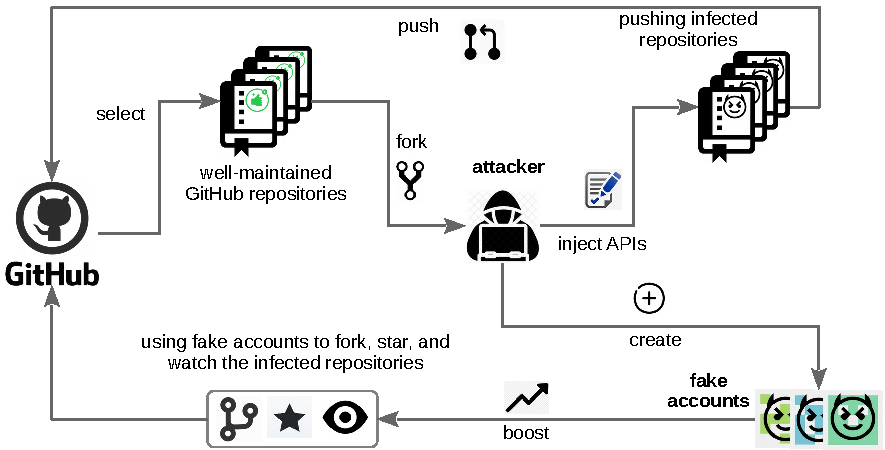
\includegraphics[width=0.450\linewidth]{figs/PushAttacks.pdf}
%	%\vspace{-.1cm}
%	\caption{Manipulating \GH to boost the visibility of malicious repositories~\cite{9678946}.} %Performing push attacks
%	\vspace{-.3cm}
%	\label{fig:PushAttacks}
%\end{figure}
%
%%Let us imagine a scenario in which one increases the popularity of malicious APIs\footnote{An API is considered as malicious if it causes fatal errors, no matter where it comes from, \ie either a legitimate or a fake library.} by planting them to OSS projects, as many as possible. 
%
%Figure~\ref{fig:PushAttacks} depicts a scenario, with which hostile users can follow to seed malicious repositories. First, attackers fork well-maintained repositories from \GH, \eg those that have good indicators with respect to the number of stars, forks, or watchers. Afterward, they inject projects with fake APIs, and then upload again to \GH. %In fact, malicious repositories are quite a phenomenon in \GH%are not scarce, but \emph{dime a dozen}
%%~\cite{Rokon2020SourceFinderFM}. 
%The visibility of a malicious API can be amplified by injecting it into a significant number of declarations for each training project. Moreover, to expose better the adversary repositories to search engines, attackers may create fake accounts to star, fork, and watch the malicious repositories.\footnote{Such manipulation has been recently revealed \url{https://zd.net/3bg3CK9}.} In fact, malicious repositories are quite a phenomenon, and many of them with malware apps have been detected in \GH \cite{Rokon2020SourceFinderFM}. %, and they might be only \emph{the tip of the iceberg}. %, waiting. 
%
%%There are precedents where thousands of repositories
%%===============================
%%Though RSSEs may choose %attempt to crawl training data from 
%%repositories considered to be \emph{credible}~\cite{NGUYEN2019110460}, \eg having a significant number of stars, forks, or watchers, unfortunately, this cannot help them completely evade toxic repositories. These metrics, however, can be falsified as attackers use fake accounts to star, fork, and watch the malicious repositories, making them appear more legitimate. Such a trick has been recently revealed, where several fake accounts are used to reciprocally endow their malicious repositories. %\footnote{\url{https://zd.net/3bg3CK9}} 
%%To our knowledge, research conducted to fight this type of abuse is still in its initial phase~\cite{10.1145/3357384.3357971}. %,Rokon2020SourceFinderFM
%%Thus, techniques to conduct attacks are known, and there are at least examples of fake repositories, albeit being created for other purposes rather than for attacking RSSE. 
%%===============================
%%Attacks may also impose different methods to hide their adversarial intent. Apart from wrapping malicious code in a single API call (see Section~\ref{sec:Example}), they might disguise it with a typosquatting name~\cite{10.1145/3463274.3463809}, \ie one that closely resembles a popular API. In this case, developers would adopt the disguised API/snippet without the least delay, once it is provided by the recommendation engine. 
%%===============================
%%increase their credibility/visibility, thus exposing them better to search engines
%%Then, based on the tool availability as well as the characteristics of the tools, 
%
%Following our main line of research in RSSEs~\cite{DBLP:journals/ese/RoccoRSNR21,NGUYEN2019110460,Nguyen:2019:FRS:3339505.3339636,10174041}, %in our recent work~\cite{9678946}, 
%by means of mixed methods research (\ie combining quantitative research and qualitative research), %mixed-method study %to a first empirical investigation 
%we shed light into the effects of adversarial machine learning in RSSEs~\cite{9678946}. Through a systematic literature review in premier software engineering venues, we found out that all of them deal with malware detection in Android apps, we did not find any work related to potential threats and implications of adversarial attacks to API RSSEs.
%%so far no existing study investigates the issue of adversarial attacks to API  recommender systems. % has not attracted attention from the research community. % major software engineering venues. 
%%First, through a literature analysis on 14 premier venues in software engineering, we show that there has been no work to study the issue of AML in RSSE. 
%%In summary, by thoroughly investigating the papers that match 
%%Using a set of keywords to filter out irrelevant studies, we realized that all of them deal with malware detection in Android apps. Instead, we did not find any work related to potential threats and implications of adversarial attacks to API RSSE.%recommender systems.
%
%
%Next, we performed an evaluation on three state-of-the-art API recommender systems, \ie \UM~\cite{Wang2013Mining}, PAM~\cite{Fowkes:2016:PPA:2950290.2950319}, and \FC~\cite{Nguyen:2019:FRS:3339505.3339636}, % 
%%underlining their risk of being manipulated by adversarial techniques. Then, we perform an empirical evaluation on three API recommenders 
%using repositories that have been injected with harmful APIs. 
%The results revealed a worrying outcome: by crafting input data to feed the systems, we succeeded in spoiling the recommendations, promoting fake/toxic API calls that can potentially harm the end users. %, \ie %. %Last but not least, we devise some possible countermeasures to cope with this type of manipulations. 
%%The results emerged from our quantitative analyses revealed that 
%%even with a small amount of artificial training data, the ratios that systems the fake APIs are always larger than 0. %, implying that clients are being provided with the fake APIs. 
%In particular, the results demonstrated that the use of PAM may be threatened by malicious attempts concealed in training data. Also for \FC, the seeded data has an adverse effect, \ie the tool is tricked into recommending to developers the toxic APIs, and source code. \UM is also not an exception, and it is prone to adversarial attacks, suggesting malicious APIs to developers.
%%We select three of them,  \ie \UM~\cite{Wang2013Mining}, PAM~\cite{Fowkes:2016:PPA:2950290.2950319}, and \FC~\cite{Nguyen:2019:FRS:3339505.3339636}. 
%%To evaluate the resilience of \UM, PAM, and \FC, we use a dataset containing Android apps' source code. %We focused on Android apps because they entail a typical scenario in which an infection can cause unwanted consequences such as data leaks.
%Altogether, we conclude that API recommender systems are likely to be exploited, and in this way they inadvertently become a \emph{trojan horse}, threatening the security of software systems. 
%
%The results of this work have been published in the proceedings of the ASE 2021 conference:% following paper:
%\vspace{-.1cm}
%\begin{itemize}
%	\item \small{\underline{Phuong T. Nguyen}, Claudio Di Sipio, Juri Di Rocco, Massimiliano Di Penta, Davide Di Ruscio ``\emph{Adversarial Attacks to API Recommender Systems: Time to Wake Up and Smell the Coffee?}'', in Proceedings of the 36th IEEE/ACM Int. Conf. on Automated Software Engineering (ASE 2021), DOI: \href{https://doi.org/10.1109/ASE51524.2021.9678946}{10.1109/ASE51524.2021.9678946}.}
%\end{itemize}
%
%\vspace{-.4cm}


%We have the following remarks:











%``\emph{}''




%\section{Goals} \label{sec:Goals}
%
%
%
%\begin{itemize}
%	\item a machine learning model to protect privacy in software engineering system.
%	\item users are reluctant to share their data.
%	\item machine learning models tailored to software engineering applications.
%\end{itemize}
%
%Fair and robust recommender systems for software engineering.

% an initial investigation of





%==========================================
%\subsection{Mining time series data in GitHub}
%
%In open-source software repositories, there exist time-series artifacts which are the result of the interaction between developers and hosting platforms, e.g., the evolution of a software project in GitHub over the course of time. %Similarly in MDE, models evolve during their lifecycle, resulting in the transformation and evolution of models. 
%Such type of data, once being properly mined, can provide developers/modelers with useful recommendations, helping them complete their tasks. 
%
%In this respect, I assume that the deployment of Machine Learning techniques such as Long Short-Term Memory recurrent neural networks (LSTM), or Encoder-Decoder LSTM allows us to mine the existing data, providing supports to developers. 
%%In this respect, ML techniques specialized
%%in dealing with sequential data are of great use, i.e., 
%These algorithms are able to learn from time series data to perform predictions for unknown sequences of events. Some initial attempts have already been made following this paradigm, achieving a promising performance.
%%For instance, Burgueño et al. [121] proposed an automatic approach to model trans-
%%formations built on top of an LSTM neural network. 
%Once trained, the systems can
%automatically transform an input model into the corresponding output without needing any transformation-specific code. Furthermore, I anticipate that the application of cutting-edge neural networks %, %such as Encoder-Decoder, or Transformer, 
%can help tackle various issues, including model transformation and model evolution, further boosting the prediction capability.
%==========================================
